%\documentclass[a4paper,12pt]{article}  % standard LaTeX, 12 point type
\documentclass[12pt, a4paper]{article}

\usepackage{algpseudocode}
\usepackage{algorithm}
\usepackage{algorithmicx}

\usepackage{geometry}
\usepackage{amsfonts,latexsym}
\usepackage{amsthm}
\usepackage{amssymb}
\usepackage[utf8]{inputenc} % Кодировка
\usepackage[english,russian]{babel} % Многоязычность
\usepackage{mathtools}
\usepackage{hyperref}
\usepackage{tikz}
\usepackage{dsfont}
\usepackage{multicol}
\usetikzlibrary{fit,calc,automata,positioning}

\theoremstyle{definition}
\newtheorem{definition}{Определение}[section]
\newtheorem{example}{Пример}[section]
\newtheorem{theorem}{Теорема}[section]
\newtheorem{proposition}[theorem]{Proposition}
\newtheorem{lemma}[theorem]{Лемма}
\newtheorem{corollary}[theorem]{Corollary}
\newtheorem{conjecture}[theorem]{Conjecture}


% unnumbered environments:

\theoremstyle{remark}
\newtheorem*{remark}{Remark}
\newtheorem*{notation}{Notation}
\newtheorem*{note}{Note}



\setlength{\parskip}{5pt plus 2pt minus 1pt}
%\setlength{\parindent}{0pt}


\algtext*{EndWhile}% Remove "end while" text
\algtext*{EndIf}% Remove "end if" text
\algtext*{EndFor}% Remove "end for" text
\algtext*{EndFunction}% Remove "end function" text


\usepackage{color}
\usepackage{listings}
\usepackage{caption}
\usepackage{graphicx}
\usepackage{ucs}

\graphicspath{{pics/}}

\geometry{left=2cm}
\geometry{right=1.5cm}
\geometry{top=2cm}
\geometry{bottom=2cm}




%\lstnewenvironment{algorithm}[1][]
%{
%    \lstset{
%        frame=tB,
%        numbers=left,
%        mathescape=true,
%        numberstyle=\small,
%        basicstyle=\small,
%        inputencoding=utf8,
%        extendedchars=\true,
%        keywordstyle=\color{black}\bfseries,
%        keywords={,function, procedure, return, datatype, function, in, if, else, for, foreach, while, denote, do, and, then, assert,}
%        numbers=left,
%        xleftmargin=.04\textwidth,
%        #1 % this is to add specific settings to an usage of this environment (for instnce, the caption and referable label)
%    }
%}
%{}

\newcommand{\tab}[1][0.3cm]{\ensuremath{\hspace*{#1}}}

\newcommand{\rvline}{\hspace*{-\arraycolsep}\vline\hspace*{-\arraycolsep}}

\newcommand{\derives}[1][*]{\xRightarrow[]{#1}}
\newcommand{\first}[1][1]{\textsc{first}_{#1}}
\newcommand{\follow}[1][1]{\textsc{follow}_{#1}}

\setcounter{MaxMatrixCols}{20}


\tikzset{
%->, % makes the edges directed
%>=stealth’, % makes the arrow heads bold
node distance=4cm, % specifies the minimum distance between two nodes. Change if necessary.
%every state/.style={thick, fill=gray!10}, % sets the properties for each ’state’ node
initial text=$ $, % sets the text that appears on the start arrow
}

\tikzstyle{symbol_node} = [shape=rectangle, rounded corners, draw, align=center]
\tikzstyle{prod_node} = [shape=rectangle, draw, align=center]

\tikzset{
    between/.style args={#1 and #2}{
         at = ($(#1)!0.5!(#2)$)
    }
}

%every node/.style = {shape=rectangle, rounded corners,
%      draw, align=center,
%      top color=white, bottom color=blue!20}

\title{Теория формальных языков. Лекции и практики. Заметки.}
\author{Семён Григорьев}
\date{\today}

\begin{document}
\maketitle
\newpage
\tableofcontents
\newpage

\section{План лекций}
\begin{enumerate}
  \item Введение. Базовые определения. Обзор курса.
  \item Регулярные языки, конечные автоматы (детерминированные, недетерминированные), регулярные выражения. Детерминизация, $\varepsilon-$замыкание, минимизация.
  \item Взаимные преобразования способов задания.
  \item Теоретико-языковые свойства регулярных языков. Лемма о накачке, замкнутость относительно операций.
  \item Алгоритмы вычисления операций.
  \item Лево(право)-линейные грамматики и регулярные языки.
  \item Грамматики, переписывающие системы. КС-граммтики (обыкновенные граммтики). Вывод в граммтике, неоднозначные грамматики, существенно неоднозначные языки, дерево вывода.
  \item Рекурсивные автоматы.
  \item Лемма о накачке, замкнутотсть относительно операций, проверка пустоты.
  \item Нормальная форма Хомского, CYK.
  \item LL
  \item LR
  \item !!!
  \item !!!
  \item !!!
  \item !!!
  \item !!!
\end{enumerate}


\section{Лекция 1: Введение}

Алфавит, язык. Операции над строками. Операции над языками.

Какие вопросы можно задавать о языках: о пустоте, универсальности, о построении пересечения, о пустоте пересечения, о вложенности, об эквивалентности.

Базовые способы задания: перечисление, генератор, распознаватель.

Грамматики. Иерархия Хомского. Проблемы с ней. Классы языков.

Взаимосвязь теории формальных языков с другими областями, области её применения.
\begin{itemize}
  \item Синтаксический анализ языков программирования: в компиляторах, интерпертаторах, средах разработки, других инстументах.
  \item Анализ естественных языков.
  Активность в этой области несколько спала, так как на передний план сейчас вышли различные методы машинного обучения.
  Однако и в этой области ведуться работы. 
  Примеры конференций: 
  \begin{itemize}
    \item \href{http://www.wikicfp.com/cfp/servlet/event.showcfp?eventid=98626&copyownerid=320}{International Conference on Parsing Technologies} (\href{https://iwpt20.sigparse.org/callforpapers.html}{IWPT-2020})
    \item \href{http://www.wikicfp.com/cfp/program?id=1029&s=FG&f=Formal%20Grammar}{FG: Formal Grammar} (\href{http://fg.phil.hhu.de/2020/}{FG-2020})
  \end{itemize}

  \item Статический анализ кода.
  \begin{itemize}
    \item Различные задачи межпроцедурного анализа. Основной подход --- language reachability. Основоположник --- Томас Репс. Примеры работ.
    \begin{itemize}
      \item Thomas Reps. 1997. Program analysis via graph reachability. In Proceedings of the 1997 international symposium on Logic programming (ILPS ’97). MIT Press, Cambridge, MA, USA, 5–19.
      \item Qirun Zhang and Zhendong Su. 2017. Context-sensitive data-dependence analysis via linear conjunctive language reachability. In Proceedings of the 44th ACM SIGPLAN Symposium on Principles of Programming Languages (POPL 2017). Association for Computing Machinery, New York, NY, USA, 344–358. DOI:https://doi.org/10.1145/3009837.3009848
      \item Kai Wang, Aftab Hussain, Zhiqiang Zuo, Guoqing Xu, and Ardalan Amiri Sani. 2017. Graspan: A Single-machine Disk-based Graph System for Interprocedural Static Analyses of Large-scale Systems Code. In Proceedings of the Twenty-Second International Conference on Architectural Support for Programming Languages and Operating Systems (ASPLOS ’17). Association for Computing Machinery, New York, NY, USA, 389–404. DOI:https://doi.org/10.1145/3037697.3037744
      \item Lu Y., Shang L., Xie X., Xue J. (2013) An Incremental Points-to Analysis with CFL-Reachability. In: Jhala R., De Bosschere K. (eds) Compiler Construction. CC 2013. Lecture Notes in Computer Science, vol 7791. Springer, Berlin, Heidelberg
    \end{itemize}
    \item Интерливинг (или шафл) языков для верификаци многопоточных программ.
    \begin{itemize}
      \item \href{http://uu.diva-portal.org/smash/get/diva2:442518/FULLTEXT01.pdf}{Approximating the Shuffle of Context-free Languages to Find Bugs in Concurrent Recursive Programs}
      \item Flick N.E. (2015) Quotients of Unbounded Parallelism. In: Leucker M., Rueda C., Valencia F. (eds) Theoretical Aspects of Computing - ICTAC 2015. ICTAC 2015. Lecture Notes in Computer Science, vol 9399. Springer, Cham
    \end{itemize}

    \item Система типов Java: \href{https://arxiv.org/abs/1605.05274}{Radu Grigore, Java Generics are Turing Complete}.
  \end{itemize}

  \item Графовые базы данных. Поиск путей с ограничениями. 
    \begin{itemize}
      \item Maurizio Nolé and Carlo Sartiani. 2016. Regular Path Queries on Massive Graphs. In Proceedings of the 28th International Conference on Scientific and Statistical Database Management (SSDBM ’16). Association for Computing Machinery, New York, NY, USA, Article 13, 1–12. DOI:https://doi.org/10.1145/2949689.2949711
      \item Jochem Kuijpers, George Fletcher, Nikolay Yakovets, and Tobias Lindaaker. 2019. An Experimental Study of Context-Free Path Query Evaluation Methods. In Proceedings of the 31st International Conference on Scientific and Statistical Database Management (SSDBM ’19). Association for Computing Machinery, New York, NY, USA, 121–132. DOI:https://doi.org/10.1145/3335783.3335791
      \item \href{https://arxiv.org/abs/1502.02242}{Jelle Hellings. Querying for Paths in Graphs using Context-Free Path Queries.}
    \end{itemize}

  \item Биоинформатика. В основном это анализ геномных и белковых последовательностей.
    \begin{itemize}
      \item \href{https://www.ncbi.nlm.nih.gov/pmc/articles/PMC6428041/}{Witold Dyrka, Mateusz Pyzik, Francois Coste, and Hugo Talibart. Estimating probabilistic context-free grammars for proteins using contact map constraints}.
      \item \href{https://www.ncbi.nlm.nih.gov/pmc/articles/PMC3464655/}{James WJ Anderson, Paula Tataru, Joe Staines, Jotun Hein, and Rune Lyngso. Evolving stochastic context-free grammars for RNA secondary structure prediction}.
      \item \href{https://www.semanticscholar.org/paper/Predicting-RNA-secondary-structure-using-a-grammar-Zier-Vogel/90bb312cb1a0f61eddb7a8b5b782bb40630894dd}{Ryan Zier-Vogel. Predicting RNA secondary structure using a stochastic conjunctive grammar.}
    \end{itemize}

  \item Машинное обучение.
   \begin{itemize}
      \item \href{https://arxiv.org/abs/1703.01925}{Matt J. Kusner, Brooks Paige, José Miguel Hernández-Lobato. Grammar Variational Autoencoder}. Опубликована в 2017 году и уже \href{https://scholar.google.com/scholar?cites=4080460899049502885&as_sdt=2005&sciodt=0,5&hl=ru}{больше 200 цитирований.}
      \item \href{https://www.aclweb.org/anthology/D17-1180.pdf}{TAG Parsing with Neural Networks and Vector Representations of Supertags}. К разговору об оброаботке естественных языков.
      \item \href{https://arxiv.org/abs/1804.06610}{Jungo Kasai, Robert Frank, Pauli Xu, William Merrill, Owen Rambow. End-to-end Graph-based TAG Parsing with Neural Networks.}
    \end{itemize}

  \item Языки --- это не только про строки.
  \begin{itemize}
    \item Языки деревьев: \href{http://tata.gforge.inria.fr/}{Tree Automata Techniques and Applications}.
    \item Языки графов: 
    \begin{itemize}
      \item \href{http://www.its.caltech.edu/~matilde/GraphGrammarsLing.pdf}{Graph Grammars}
      \item \href{https://people.cs.umu.se/drewes/biblio/ps-files/hrg.pdf}{HYPEREDGE REPLACEMENT GRAPH GRAMMARS}
      \item \href{https://www.aclweb.org/anthology/W17-3410.pdf}{(Re)introducing Regular Graph Languages}
      \item \href{https://www.springer.com/gp/book/9783540560050}{Hyperedge Replacement: Grammars and Languages}
    \end{itemize}
    \item $\ldots$
  \end{itemize}
  \item Теория групп. Как правило, это проблема слов группы или дополнение к ней.
  \begin{itemize}
    \item Anisimov, A.V. Group languages. Cybern Syst Anal (1971) 7: 594.
    \item David E. Muller, Paul E. Schupp, Groups, the Theory of ends, and context-free languages, Journal of Computer and System Sciences, Volume 26, Issue 3, 1983, Pages 295-310, ISSN 0022-0000
    \item HOLT, D., REES, S., ROVER, C., \& THOMAS, R. (2005). GROUPS WITH CONTEXT-FREE CO-WORD PROBLEM. Journal of the London Mathematical Society, 71(3), 643-657. doi:10.1112/S002461070500654X
    \item \href{https://arxiv.org/abs/1407.7745}{Groups with Context-Free Co-Word Problem and Embeddings into Thompson's Group V} 
    \item \href{https://www.degruyter.com/view/j/gcc.2019.11.issue-1/gcc-2019-2004/gcc-2019-2004.xml}{Kropholler, R. \& Spriano, D. (2019). Closure properties in the class of multiple context-free groups. Groups Complexity Cryptology, 11(1), pp. 1-15. Retrieved 13 Feb. 2020, from doi:10.1515/gcc-2019-2004}
    \item \href{https://personalpages.manchester.ac.uk/staff/Mark.Kambites/events/nbsan/nbsan17_thomas.pdf}{Word problems of groups, formal languages and decidability}
  \end{itemize}

  \item Прочая забавная математика.
  \begin{itemize}
    \item Немного топологии в теории формальных языков: \href{https://hal.archives-ouvertes.fr/hal-01771670/}{Salvati S. On is an n-MCFL. – 2018.}
    \item Salvati S. MIX is a 2-MCFL and the word problem in Z2 is captured by the IO and the OI hierarchies //Journal of Computer and System Sciences. -- 2015. -- Т. 81. -- \textnumero. 7. -- С. 1252-1277.
    \item О том, как задачи из теории графов связаны с теорией формальных языков: Abboud, Amir \& Backurs, Arturs \& Williams, Virginia. (2015). If the Current Clique Algorithms are Optimal, So is Valiant's Parser. 98-117. 10.1109/FOCS.2015.16.
    \item \href{https://www.sciencedirect.com/science/article/abs/pii/S0196885819300739}{A context-free grammar for the Ramanujan-Shor polynomials}
  \end{itemize}
\end{itemize}

\section{Практика 1}

Детали о том, как будет проходить практика.

\subsection{Григорьев С.В.}

Немного про описания языков.
Пописать языковые уравнения, граммтики.
Посмотреть на операции над языками.

Постановка задачи на весь семестр.

Запросы к графовым базам данных.
Контекст задачи, примеры графовых БД (RedisGraph, Neo4j, ...), задача о путях впринципе.

Ссылка на второй конспект.

Задача: реализовать свою "графовую миниБД".

Реализация: оформление, инструменты, языки.

\begin{itemize}
  \item Ограничений на язык реализации нет.
  \item Ограничений на использование библиотек нет. Главное --- не нарушать лицензии и чтобы можно было вносить изменения в библиотеку (при необходимости).
  \item Каждый создёт под решение репозиторий на GitHub и снабжает его всем необходимым: readme, лицензия, CI-сборка с тестированием, инструкции по локальному развёртыванию.
  \item Разработка ведётся в отдельной ветке и когда очередная часть задачи готова к сдаче --- делаем pull request в master и добавляем меня (gsvgit) в ревьюверы.
\end{itemize}


Задачи на дом.
\begin{enumerate}
  \item Выбрать язык программирования, на котором будет вестись разработка.
  \item Создать репозиторий на GitHub.
  \item Настроить CI-сборку и тестирование.
  \item Реализовать подгрузку графов из RDF используя готовые библиотеки.
\end{enumerate}


\section{Лекция 2}

\subsection{Первое знакомство с F\#}

    Общие сведения о платформе .NET, общие представления об архитектуре платформы.

    F\# --- это один из языков платформы. 
    Некоторые ресурсы дл того, чтобы начать изучать F\#.
    \begin{itemize}
    	\item Главный сайт сообщества: \url{https://fsharp.org/}. Там много чего интересного, от библиотек и инструментов до ссылок на другие ресурсы. 
    	\item Неплохая книга по основам языка: \url{https://en.wikibooks.org/wiki/F_Sharp_Programming}
    	\item Подборка обучающих материалов от сообщества: \url{https://fsharp.org/learn/}
    	\item Официальная документация от Microsoft: \url{https://docs.microsoft.com/ru-ru/dotnet/fsharp/}
    \end{itemize}
    Основные особенности F\#, примеры кода, базовые языковые конструкции и типы.

    Примитивные типы: логисекие, числовые, символы, строки.
    Массивы, основные функции работы с ними: инициализация, взятие элемента, запись элемента.

    Базовые констукции управления: ветвления (if), циклы (различные варианты for, while). 
    Двумерный синтаксис.

    Структура программы. Точка входа, модули, функции. Модуль и пространство имён.

    Основы работы с консолью, библиотека \href{https://fsprojects.github.io/Argu/}{Argu}. 

\subsection{Тестирование программ}
    Тестирование программ: ручное, автоматизированное, автоматическое. 

    Доказательство корректности vs тестирование. Тестирование не есть доказательство корректности.
    А можно ли всё таки доказать корректность? Да (иногда).
    \begin{itemize}
    	\item \href{https://en.wikipedia.org/wiki/Formal_verification#Formal_verification_for_software}{Формальная верификация} используя внешние инструменты.
        \item Использование специальных языков программирования, таких как \href{https://coq.inria.fr/}{Coq} (на самом деле это целая система, так называемый proof assistant), \href{https://wiki.portal.chalmers.se/agda/pmwiki.php}{Agda}, \href{https://www.idris-lang.org/}{Idris}, \href{https://www.fstar-lang.org/}{F*},   
    \end{itemize}

    Типы тестов и особенности их применения: модульные, интеграционные, unit и т.д. Автоматизация создания тестов. \href{https://docs.microsoft.com/en-us/visualstudio/test/intellitest-manual/?view=vs-2019}{Intellitest} --- пример инстумента для автоматической генерации тестов. Примеры инструментов для тестирования: \href{https://github.com/haf/expecto}{Expecto}, \href{http://fsprojects.github.io/FsUnit/index.html}{FsUnit}, \href{https://nunit.org/}{NUnit}, \href{https://fscheck.github.io/FsCheck/}{FsCheck}, \href{http://lefthandedgoat.github.io/canopy/}{Canopy}. 

    С этого момента все домашние работы должны быть снабжены автоматически запускаемыми при сборке тестами.

\section{Практика 2}

\subsection{Григорьев С.В.}

Построение ДКА по регулярному варажению.
Парсер регулярных выражений. Немного про AST и прочее.

Пересечение ДКА и НКА (без $\varepsilon$-переходов): библиотека и руками через произведение Кронекера (прямое произведение). Сравнение производительности.

Представление результата в виде графа и регулярного выражения.







\section{Лекция 3}

	Ещё раз произменения: в реквесте должно быть только то, что непосредственно относится к сдаваемой домашке.

	Ещё раз про функции, про то, как выделять и разделять функциональность, не надо запихивать всё в одну функцию. Про то, где должны быть проверки.

	Про консоль.

	Про обработку крайних случаев. Про исключения.

	Про тесты и ошибки: нашёл ошибку --- создал тест.

	Про стиль кодирования: про пробелы вокруг скобок и операций, про отступы и переводы строк. Про соглашения о наименовании. camlCase CamlCase


	Про единицы измерения.

    Базовые структуры данных, алгоритмы и их выражение в F\#. Функция. Рекурсия и итерация.  Базовые типы и основы работы с ними: матрицы, массивы, списки, структуры. 


    Числа Фибоначчи.
\section{Практика 3}

\subsection{Григорьев С.В.}

Пересечение автоматов --- это тензорное произведение матриц смежности. Пример.

Про коммутативность пересечения и некоммутативность тензорного произведения.

Домашнее задание.
\begin{enumerate}
	\item Реализовать консольный клиент, позволяющий
	\begin{enumerate}
		\item загрузить RDF-файл
		\item вывести список меток рёбер
		\item задать к загруженному графу регулярный запрос с возможностью указать представление результата: пустота ответа, автомат сдампить в файл в формате DOT (\url{https://www.graphviz.org/doc/info/lang.html}), пара (кол-во рёбер, кол-во вершин) в результирующем автомате
	    \item выйти из клиента.
    \end{enumerate}
	\item Подгрузку RDF и выполнение запросов реализовать на основе уже существующей функциональности.
	\item Провести замеры производительности на графах из репозитория \url{https://github.com/JetBrains-Research/CFPQ_Data}. Графы брать из подпапки \verb|data/graphs/RDF|. Так как в графах присутствуют одинаковые отношения, то можно один и тот же запрос выполнять на всех графах. Отчёт оформить в виде раздела в  README репозитория в виде таблицы. 

	\textit{Эти эксперименты проводятся локально! Не надо таскать репозиторий с графами за собой. Для тестов клиента использовать маленькие синтетические RDF.}
	\item Реализовать необходимые тесты на работоспособность клиента.
\end{enumerate} 

\section{Лекция 4}

Рекурсивные автоматы. Построение, интерпретация.


\section{Практика 4}

\subsection{Григорьев С.В.}

Больше подробностей про рекурсивные автоматы: тотальная минимизация. Как их приментять для КС запросов. Тензоры + транзитивное замыкание.

Домашнее задание.
\begin{enumerate}
	\item Реализовать выполнение регулярных щапросов через тензорное произведение. Для тензорного произведения использовать существующие библиотеки линейной алгебры. Обратите внимание на то, что матрицы должны быть разреженными. Скорее всего, удобно будет использовать представление в виде набора булевых матриц.
	\item Интегрировать новую реализацию в клиент наравне со старой.
	\item Провести замеры производительности на графах из репозитория \url{https://github.com/JetBrains-Research/CFPQ_Data}. Графы брать из подпапки \verb|data/graphs/RDF|. Так как в графах присутствуют одинаковые отношения, то можно один и тот же запрос выполнять на всех графах. Отчёт оформить в виде раздела в  README репозитория в виде таблицы. Сравнить с результатми предыдущей задачи. 

	\textit{Эти эксперименты проводятся локально! Не надо таскать репозиторий с графами за собой. Для тестов клиента использовать маленькие синтетические графы и запросы.}
	\item Реализовать необходимые тесты на работоспособность алгоритма через тензорное произведение.
\end{enumerate} 


\section{Лекция 5}
 
\subsection{Нормальня форма Хомского (НФХ)}

\begin{definition}
КС грамматика находится в нормальной форме Хомского если любое правило имеет один из трёх видов:
\begin{enumerate}
    \item $S \to \varepsilon$
    \item $N_i \to t_j$
    \item $N_i \to N_j N_k$, $N_j \neq S, N_k \neq S$
\end{enumerate}
\end{definition}
Важно: стартовый нетерминал не встречается в правых частях правил, $\varepsilon$-продукция только для стартового нетерминала.

\begin{note}
Любую КС грамматику можно преобразвать к нормальной форме Хомского.
\end{note}

Преобразование в НФХ. Шаги.
\begin{enumerate}
    \item Устранение длинных правил.
    \item Устранение $\varepsilon$-правил.
    \item Устранение цепных правил.
    \item Устранение бесполезных нетерминалов
    \begin{enumerate}
        \item Удаление непорождающих нетерминалов
        \item Удаление недостижимых нетерминалов
    \end{enumerate}
    \item Устранение продукций с правой частью длины 2, содержащей терминалы. 
\end{enumerate}

Надо не забыть добавить новый стартовый нетерминал, если нужно: чтобы вывести из него $\varepsilon$ и чтобы не встречался в правых частях правил. 

\textbf{Важно.}
Порядок применения шагов преобразования важен.
\begin{enumerate}
    \item Второй шаг можно поднять наверх, но это приведёт к более существенному разростанию результирующей граммтики.
    \item Подшаги шага 4 нельзя менять местами. Попробуйте поприменять их к граммтике:

\begin{align*}
S \to & A B \mid a \\
A \to & b
\end{align*}
    
\end{enumerate}

\href{https://neerc.ifmo.ru/wiki/index.php?title=%D0%9D%D0%BE%D1%80%D0%BC%D0%B0%D0%BB%D1%8C%D0%BD%D0%B0%D1%8F_%D1%84%D0%BE%D1%80%D0%BC%D0%B0_%D0%A5%D0%BE%D0%BC%D1%81%D0%BA%D0%BE%D0%B3%D0%BE}{Материалы по преобразованию в НФХ.}


\subsection{Лемма о накачке для КС языков}

\begin{theorem}
Пусть $L$ --- контекстно-свободный язык над алфавитом $\Sigma$, тогда существует такое $n$, что для любого слова $\omega \in L$, $|\omega| \leq n$ найдутся слова $u,v,x,y,z\in \Sigma^*$, для которых верно: $uvxyz = \omega, vy\neq \varepsilon,|vxy|\leq n$ и для любого $k \geq 0$  $uv^kxy^kz \in L$.
\end{theorem}

Идея доказательства леммы о накачке.

\begin{enumerate}
    \item Для любого КС языка можно найти грамматику в нормальной форме Хомского.
    \item Очевидно, что если брать достаточно длинные цепочки, то в дереве вывода этих цепочек, на пути от корня к какому-то листу обязательно будет нетерминал, встречающийся минимум два раза. Если $m$ --- количество нетерминалов в НФХ, то длины $2^{m+1}$ должно хватить. Это и будет $n$ из леммы.
    \item Возьмём путь, на котором есть хотя бы дважды повторяется некоторый нетерминал. Скажем, это нетерминал  $N_1$. Пойдём от листа по этому пути. Найдём первое появление $N_1$. Цепочка, задаваемая поддеревом для этого узла --- это $x$ из леммы.
    \item Пойдём дальше и найдём второе появление $N_1$. Цепочка, задаваемая поддеревом для этого узла --- это $vxy$ из леммы.
    \item Теперь мы можем копировать кусок дерева между этими повторениями $N_1$ и таким образом накачивать исходную цепочку.
\end{enumerate}

Надо только проверить выполение ограничений на длины.

\begin{figure}
\centering
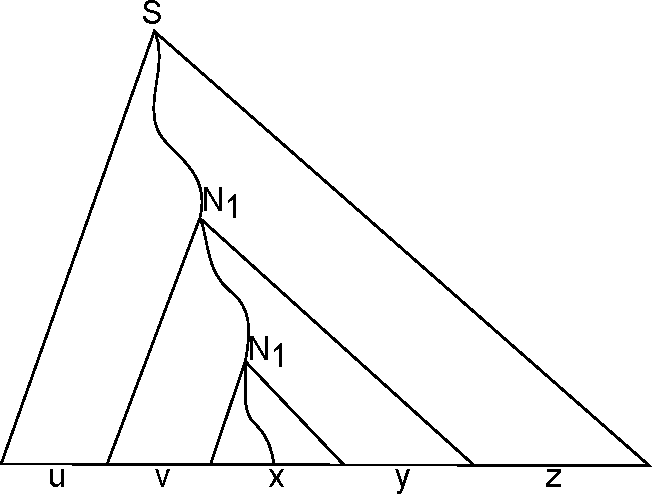
\includegraphics[width=0.5\textwidth]{figures/pumping_tree_1.pdf}
\caption{Разбиение цепочки для леммы о накачке}
\label{fig:pumping1}
\end{figure}

\begin{figure}
\centering
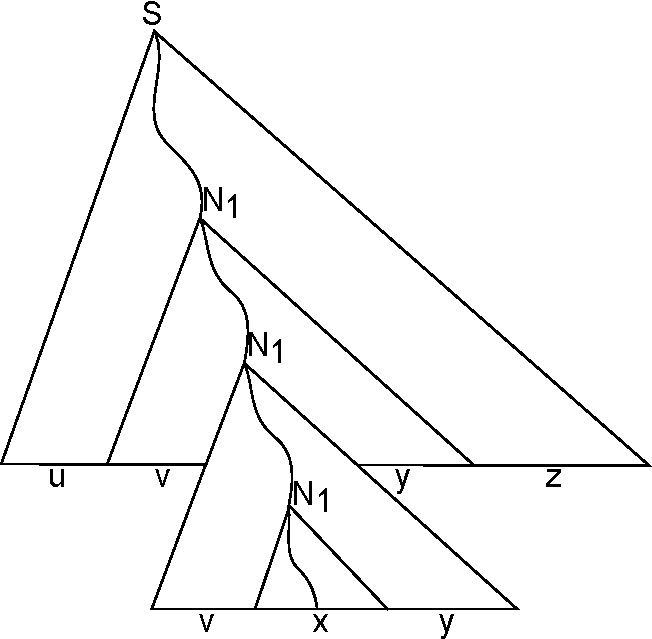
\includegraphics[width=0.5\textwidth]{figures/pumping_tree_2.pdf}
\caption{Пример накачки цепочки с рисунка~\ref{fig:pumping1}}
\end{figure}


\href{https://neerc.ifmo.ru/wiki/index.php?title=%D0%9B%D0%B5%D0%BC%D0%BC%D0%B0_%D0%BE_%D1%80%D0%B0%D0%B7%D1%80%D0%B0%D1%81%D1%82%D0%B0%D0%BD%D0%B8%D0%B8_%D0%B4%D0%BB%D1%8F_%D0%9A%D0%A1-%D0%B3%D1%80%D0%B0%D0%BC%D0%BC%D0%B0%D1%82%D0%B8%D0%BA}{Материалы по лемме о накачке для КС языков.}

Проверить неконтекстно-свободность языка $L=\{a^nb^nc^n \mid n>0\}$.

\section{Домашняя работа 5}

В данной задаче предолагается, что для обработки сырых данных и отрисовки графиков используется Python и Matplotlib, однако другие сравнимые по выразительности и качеству результата пакеты разрешены. Исользование офисных пакетов (типа LibreOffice, MS Office и т.д.) запрещено. Шрафики должны быть векторными. Внимательно ледите за тем, что в репозиторий должны быть только исходники, сгенерированные файлы в репозиторий попасть не должны.

\begin{enumerate}
    \item \textbf{(5 баллов)} Провести сравнительное исследование реализованных в предыдущей домашней работе сортировок и стандартных реализаций сортировок соответствующих коллекций. Оформить отчёт: введение, детали реализации, постановка эксперимента, результаты экспериментов, анализ результатов. Отчёт оформляется в \LaTeX, исходники выкладываются так же как и обычный код, снабжаются скриптом сборки (Shell), который генерирует графики и собирает pdf-документ.
\end{enumerate}


\bibliographystyle{abbrv}
\bibliography{Formal_language_course}


\end{document}
